%!TEX TS-program = xelatex 
%!TEX TS-options = -synctex=1 -output-driver="xdvipdfmx -q -E"
%!TEX encoding = UTF-8 Unicode
%
%  my_title
%
%  Created by my_name on date.
%  Copyright (c) year. All rights reserved.
%

\documentclass[12pt]{article} 

% Definitions
\newcommand\mykeywords{color, illusion} 
\newcommand\myauthor{Mark Eli Kalderon} 
\newcommand\mytitle{Color Illusion}

% Packages
\usepackage{geometry} \geometry{a4paper} 
\usepackage{url}
\usepackage{txfonts}
\usepackage{color}
\definecolor{gray}{rgb}{0.459,0.438,0.471}
% \usepackage{setspace}
% \doublespace % Uncomment for doublespacing if necessary
\usepackage{epigraph} % optional

% XeTeX
\usepackage[cm-default]{fontspec}
\usepackage{xltxtra,xunicode}
\defaultfontfeatures{Scale=MatchLowercase,Mapping=tex-text}
\setmainfont{Palatino}
\setsansfont{Gill Sans}
\setmonofont{Inconsolata}

% Section Formatting
\usepackage[]{titlesec}
\titleformat{\section}[hang]{\fontsize{14}{14}\scshape}{\S{\thesection}}{.5em}{}{}
\titleformat{\subsection}[hang]{\fontsize{12}{12}\scshape}{\S{\thesubsection}}{.5em}{}{}
\titleformat{\subsubsection}[hang]{\fontsize{12}{12}\scshape}{\S{\thesubsubsection}}{.5em}{}{}

% Headers and Footers
\usepackage{fancyhdr}
\pagestyle{fancy}
\pagenumbering{arabic}
\lhead{\thepage}
\chead{}
\rhead{\itshape{\nouppercase{\leftmark}}}

% TODO List
\usepackage{color}
\usepackage{index} % use index package to create indices
\newindex{todo}{tod}{tnd}{TODO List} % start todo list
\newindex{fixme}{fix}{fnd}{FIXME List} % start fixme list
\newcommand{\todo}[1]{\textcolor{blue}{TODO: #1}\index[todo]{#1}} % macro for todo entries
\newcommand{\fixme}[1]{\textcolor{red}{FIXME: #1}\index[fixme]{#1}} % macro for fixme entries

% Bibliography
\usepackage[round]{natbib} 

% Title Information
\title{\mytitle} % For thanks comment this line and uncomment the line below
%\title{\mytitle\thanks{}}% 
\author{\myauthor} 
% \date{} % Leave blank for no date, comment out for most recent date

% PDF Stuff
\usepackage[plainpages=false, pdfpagelabels, bookmarksnumbered, backref, pdftitle={\mytitle}, pagebackref, pdfauthor={\myauthor}, pdfkeywords={\mykeywords}, xetex, dvipdfmx, colorlinks=true, citecolor=gray, linkcolor=gray, urlcolor=gray]{hyperref} 



%%% BEGIN DOCUMENT
\begin{document}

% Title Page
\maketitle

\begin{abstract} % optional
	\noindent As standardly conceived, an illusion is an experience of an object \( o \) appearing \( F \) where \( o \) is not in fact \( F \). Paradigm examples of color illusion, however, do not fit this pattern. A diagnosis of this uncovers different sense of appearance talk that is the basis of a dilemma for the standard conception. The dilemma is only a challenge. But if the challenge cannot be met, then any conception of experience, such as representationalism, that is committed to the standard conception is false. Perhaps surprisingly, naïve realism provides a better account of color illusion.
\end{abstract} 

\vskip 2em \hrule height 0.4pt \vskip 2em

\epigraph{An apparence ymaad by som Magyk.}{\textsc{Chaucer}} 

% Layout Settings
\setlength{\parindent}{1em}

% Main Content

\section{Introduction} % (fold)
\label{sec:introduction}

I have lost my grip on what color illusion is meant to be. Perhaps I have simply lost my grip---not an alternative to be ruled out in advance of inquiry. However, I believe that there is an alternative explanation. I have come to suspect that there is nothing answering to the philosopher's conception of illusion. That is not to say that there are no color appearances that might, with propriety, be described as illusory. There is a familiar genre of books illustrating optical illusions, many essentially involving chromatic phenomena. No charge of false advertising is leveled here. It is only a distinctively \emph{philosophical} conception of illusion whose claims are exaggerated. Or so I have, lately, come to suspect.

As standardly conceived, an illusory appearance is a state of appearing. Specifically, an illusion is an experience of an object \( o \) appearing \( F \) where \( o \) is not in fact \( F \). Given this, a color illusion will be described by a true instance of this schema that results from substituting a color adjective in for the schematic letter \( \ulcorner F \urcorner \). The simplicity of the standard conception can mask its philosophical character. It can seem to be no more than a minor regimentation of a notion familiar from ordinary life. The standard conception, however, is not without substantive philosophical content.

First, in understanding appearances in terms of states of appearing, it is committed to phenomenalism about appearances. Facts about the appearance of an object are to be explained in terms of facts about actual and possible experiences in which that object appears. So an object's appearance is how it \emph{does} or \emph{would} appear to a subject who experiences that object. In this way, phenomenalism about appearances parallels, without entailing, classical phenomenalism. While most philosophers now reject classical phenomenalism \citep[though see][]{Foster:00ny}, many accept, as an unargued assumption, that appearances are to be understood in terms of states of appearing. (Compare this with Price's \citeyear{Price:1952ix} claim that Britton's \citeyear{Britton:1926zm} conception of appearance is similarly phenomenalist.)

Not only is the standard conception committed to phenomenalism about appearances, but it is also committed to a conception of how an object appears in experience. On the standard conception of illusion, if \( o \)'s appearing \( F \) in \( S \)'s experience of \( o \) is illusory, then appearance and reality \emph{conflict}. So \( o \) must appear in \( S \)'s experience in a way that conflicts with \( o \)'s not being \( F \). In \( o \) appearing \( F \), \( S \)'s experience of \( o \) presents \( o \) as being a way that \( o \) is in fact not. So conceived, \( F \) qualifies \( o \). \( F \) is a way for things to be, even if it is way nothing could be (as when we are presented with an impossible scene such as Penrose's \citeyear{Penrose:1958kx} impossible triangle or a scene depicted by an Escher drawing.). And the quality designated by \( \ulcorner F \urcorner \) is attributed in experience to the object seen.

There are two ways to understand this conflict, depending on whether experience is understood to be presentational or representational. Experience is intentional, at least in the sense that it is \emph{of} or \emph{about} an encounterable aspect of the material environment. To be intentional in this minimal sense is for experience to have an object or subject matter. Even sense-datum theorists, naïve realists, and disjunctivists can accept that experience, or at least perception, is intentional in this minimal sense. The object of perceptual experience is what that experience presents. Representationalists go beyond the commitment to experiences being states of a subject that take an object and explain the intentional character of experience by attributing to experience a representational content. So, for \( o \) to appear \( F \) to a subject \( S \) is for \( S \) to undergo an experience that represents \( o \) as \( F \). 

Suppose that in the experience of \( o \) appearing \( F \), the experience involves the presentation of something which is \( F \). Since \( o \) is not \( F \), then by Leibniz's Law what is presented could not be \( o \), but some other object. Or so goes the argument from illusion. By such reasoning, the sense-datum theorist argues that what is presented in experience is not an ordinary material objects but an immaterial sense datum.  In experiencing \( o \) as \( F \), \( S \) is presented with, not \( o \), but a sense datum corresponding to \( o \). \( S \) sees \( o \) by \( S \)'s experience presenting a sense datum that corresponds to \( o \).  That sense datum is a way that \( o \) is not, namely \( F \). \( F \) is a way for things to be, it is just that it is not a way that \( o \) in fact is. The conflict, then, is between the way \( o \) is and the way the sense datum that corresponds to \( o \) is---the sense datum is \( F \) and \( o \) is not \( F \). 

Most contemporary philosophers, however, are skeptical about sense data \citep[though see][]{robinson94}. If on the standard conception of illusion there really is a conflict between appearance and reality, then the conflict is, perhaps, better understood as a conflict between the way experience represent things to be and the way things really are. So, for \( o \) to appear \( F \) to a subject \( S \) is for \( S \) to undergo an experience that represents \( o \) as \( F \). Veridical experiences are experiences with true representational contents and nonveridical experiences are experiences with false representational contents. An illusory experience is a species of nonveridical experience. In illusory experience, \( o \) is there to be encountered in \( S \)'s environment, it is just that \( S \)'s experience \emph{misrepresents} \( o \) as \( F \)---\( o \) exists, it is just that \( o \) is not \( F \) as \( S \)'s experience represents it to be. Reflection on the standard conception of illusion naturally motivates this representationalist conception of experience. On the standard conception, an illusion is an experience of an object \( o \) appearing \( F \) where \( o \) is not in fact \( F \). The subject's experience could not be a presentation of something which is \( F \)---pace, the sense-datum theorist, there is no such thing. So \( o \)'s appearing \( F \) is not the \emph{presentation} of something which is \( F \), but, at best, a \emph{representation} of something which is \( F \), since it is of the nature of representation that we can represent what is not the case. So it is natural to conclude more generally that the object or subject matter of the experience is what that experience represents.

So despite the fact that the standard conception of illusion is often regarded as minor regimentation of an ordinary notion, it is not without substantive philosophical content: It is committed to phenomenalism about appearances and naturally, if not inexorably, motivates a representationalist conception of experience. The simplicity of the standard conception may mask its philosophical content, but, by the same token, it is its very simplicity that belies its philosophical character. It is \emph{too} simple. To bring this out, we will consider paradigm examples of color illusions. Careful reflection on these reveal that they do not conform to the standard conception of illusion. I am inclined to believe that nothing does.

% section introduction (end)

\section{Benham's Disk and Pointillism} % (fold)
\label{sec:benham_s_disk}

Let's begin by considering an example of a color illusion often cited by philosophers---the subjective colors of the Benham disk.

In 1894, an English toymaker, Charles Benham, devised a top adorned with a black and white pattern (see Figure~\ref{fig:benham}). Sold through Messrs. Newton and Co., an announcement of the ``Artificial Spectrum Top'' was published in \emph{Nature}:
	\begin{quote}
		The top consists of a disc, one half of which is black, while the other half has twelve arcs of concentric circles drawn upon it. Each arc subtends an angle of forty-five degrees. In the first quadrant there are three such concentric arcs, in the next three more, and so on; the only difference being that the arcs are parts of circles of which the radii increase in arithmetical progression. Each quadrant thus contains a group of arcs differing in length from those of the other quadrants. The curious point is that when this disc is revolved, the impression of concentric circles of different colors is produced upon the retina. If the direction of rotation is reversed, the order of these tints is also reversed. \citep{Benham:1894kx}
	\end{quote}
Specifically, if rotated clockwise, the innermost arcs form reddish rings, the next greenish rings, the next light blue rings, and the outermost arcs form violet rings. If rotated counterclockwise, the pattern is reversed with the innermost arcs now forming violet rings and the outermost reddish rings. The apparent colors of Benham's spinning disk are the ``subjective colors'' first described by \citep{Fechner:1838vn} and, hence, are also sometimes described as ``Fechner-Benham colors''. 

\begin{figure}[htbp]
	\centering
		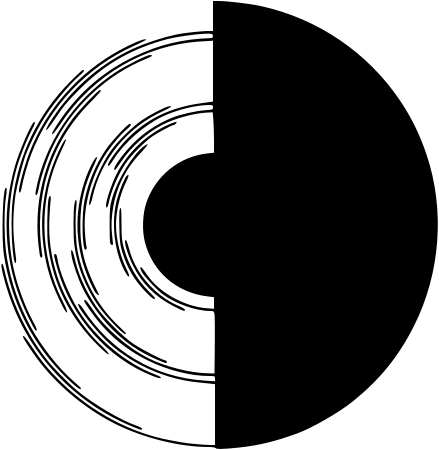
\includegraphics[scale=.5]{graphics/benhams_disk.jpg}
	\caption{Benham's Disk}
	\label{fig:benham}
\end{figure}

The subjective colors of the Benham disk are usually reckoned to be illusory. The surface of the disk is painted black and white. Nothing is black and white all over and has parts that are reddish, greenish, light blue, and violet. So these apparent colors are merely apparent. In experiencing the reddish ring, for example, we are perceiving something which is, in fact, not at all reddish. To that extent at least, the reddish appearance is \emph{illusory}. Similar reasoning holds for each of the subjective colors produced by the spinning disk.

It would seem, then, that the subjective colors produced by the Benham disk are straightforward examples of color illusions as standardly conceived. If part of Benham's spinning disk appears reddish when it is not in fact reddish, an experience presenting that appearance is illusory. So what is the problem? To bring out the problem, I want to compare the subjective colors produced by the Benham disk with the apparent colors produced by pointillist paintings.

Michel Eugène Chevreul, a French chemist appointed by Louis \textsc{xvii} as the director of the dye department of Manufacture Royale des Gobelins, upon receiving complaints that the black dyes they produced looked different when used alongside blue dye, investigated the matter and discovered the phenomena of simultaneous color contrast---that the appearance of a color can vary as the color of the surrounding scene varies. \citet{Chevreul:1855kx} reported his findings in his book, \emph{The Principles of Harmony and Contrast of Colours and Their Application to the Arts}, a book that influenced the work of the French painter Georges-Pierre Seurat. Fascinated by the appearance of a color being influenced by adjacent colors, Seurat eventually paints the pointillist masterpiece, “Un dimanche après-midi à l'Île de la Grande Jatte” in 1884--6. Using only primary unblended pigments, including the newly available zinc yellow, these were distributed in small dots across the surface of the canvas giving rise to the appearance, at an appropriate distance, of a differently colored scene of Parisian suburbanites relaxing by the river Seine.

Imagine, then, viewing a minimalist painting in a gallery. From your current vantage point, the surface of the painting appears a uniform if luminous green. Closer inspection is revealing, however. As you move in for a closer look, the painting is discovered to be not only minimalist, but pointillist. The luminous green appearance of the surface was achieved by painstakingly painting minute yellow and blue dots across the surface. In fact no part of the surface of the canvas is painted green---every part of the surface is painted either yellow or blue. Nothing is uniformly green all over and partly yellow and partly blue. One might be tempted to conclude that the green appearance of the painting is illusory. If no part of the surface of is painted green, then how could the green appearance be veridical? It would seem that we have here reasoning that straightforwardly parallel's the reasoning that convicted the subjective colors of being illusory.

Not only is there a formal analogy in the reasoning to the conclusion that the relevant appearance is illusory, but there is a material analogy as well between the cases. Consider a puzzling aspect of the subjective colors of the Benham disk. Each of the spinning arcs reflect light with the same spectral content and with equal average luminance. In advance of observing the spinning disk, one might reasonably expect the spinning arcs to appear as gray rings of equal brightness. Why, then, do the rings appear reddish, greenish, light blue, and violet? The subjective colors of the Benham disk are not completely understood \citep[for a review of some of the color science see][]{Campenhausen:1995yq}. However, this much is clear: The innermost ring appearing reddish is the result of the visual system visually integrating temporal inhomogeneities presented by the spinning disk. The case of the pointillist painting is analogous: The painting appearing green is due to the visual system visually integrating spatial inhomogeneities presented by the multicolored surface. (See \citealt[71--72]{Hardin:1993kn} and \citealt[156--158]{Johnston:1992ck})

However, as Hilbert's \citeyear{Hilbert:1987jq} discussion of Berkeley's \citeyear{Berkeley:1734fk} argument from microscopes reveals, the reasoning in the case of the pointillist painting is unsound.

% section benham_s_disk (end)

\section{The Argument from Microscopes}\label{sub:the_argument_from_microscopes} % (fold)

In arguing against the claim that ``the colors which we see exist in external bodies'', \citet{Berkeley:1734fk} presents the argument from microscopes. Consider the version of the argument that \citet{Hilbert:1987jq} adapts from \citet{Marc-Wogau:1968kx}. A drop of fresh blood looks uniformly red to the naked eye. However, as \citet[book 2, chapter 23, section 11]{Locke:1706hc} observed, ``Blood to the naked eye appears all red; but by a good microscope, wherein its lesser parts appear, shows only some few globules of red, swimming in a pellucid liquor.'' These appearances seemingly conflict---nothing can be uniformly red all over and partly red and partly transparent. If the conflict is genuine, then the Berkelean conclusion follows: Either the appearance of the drop of blood to the naked eye is illusory or the appearance of the blood through the microscope is. 

However, as \citet{Hilbert:1987jq} observes, no genuine conflict is generated. It is not that the exclusion principle---that nothing can be uniformly red all over and partly red and partly transparent---is false, only that it has no present application. There is no one thing that appears red all over and partly red and partly transparent. A drop of blood may look red to the naked eye, but we do not see the drop of blood under the microscope---we see only a proper part of it. To generate a conflict in appearance, the argument from microscopes needs to appeal to a different principle. Specifically, if what is viewed under the microscope is a proper part of the drop of blood, to generate a conflict we would need to assume that if something is colored, then all of its parts must have the same color. We would need to assume that color is \emph{dissective} in something like Goodman's \citeyearpar[53]{Goodman:1951ww} sense of the term. If color is dissective, then if the drop of blood is red, then so must all of its parts. Since the part of the blood viewed under a microscope is partly red and partly transparent, then either the appearance of the blood to the naked eye is illusory, or the appearance of the blood through the microscope is.

Are colors genuinely dissective? Goodman himself denies that they are:
\begin{quote}
	Different perceptible parts of any object may be differently colored even if the object itself is uniform and unvarying in color. This is no more paradoxical than the fact that a single object contains spatiotemporally different parts. As the self-identical object is a function of its parts, so the single unchanging color of the object is a function of the colors of its parts. The nature and interrelation of the lesser elements that make up the whole determine what kind of thing the whole is: the kind and arrangement of the colors exhibited by these various parts determine what color the whole is said to have. \citep[130]{Goodman:1951ww}
\end{quote}
In tacitly assuming that color is dissective, Berkeley seems to be assuming that once we have seen an object to be a certain color, we have seen all that there is to see about its color, including the color of its parts. This, however, flies in the face of a modest and attractive picture of perception as providing only a partial perspective on the material environment. If perception is partial, then what is seen depends not only on what there is to see, but on the visual sensibility of the perceiver and the circumstances of perception. In seeing the scene before us, the scene is presented to our partial perspective on that scene. The visible aspects of the scene is not wholly determined by any given perception of it---other perspectives may reveal further visible aspects of that scene. It is this commitment to perception providing a partial perspective on the material environment, that leads Hilbert to describe Berkeley's argument from microscopes as committing the ``fallacy of total information''. In effect, Berkeley fallaciously reasons from our failing to perceive, from a particular perspective, that the drop of blood has transparent parts, to our perceiving, from that perspective, that no part of the blood is transparent.

A weaker principle is consistent with perception being partial:
	\begin{quote}
		If from a particular perspective, as determined by the visual sensibility of the perceiver and the circumstances of perception, an object is seen to be a uniform color, then all of the parts of the object that are visible from that perspective have that color.
	\end{quote}
However, this weaker principle is insufficient to generate a conflict in appearance. The ``pellucid'' parts of the blood are not visible to the naked eye. And if no conflict is generated, then the Berkelean conclusion fails to follow.

% section the_argument_from_microscopes (end)

\section{The Benham Disk and Pointillism Revisited}\label{sub:pointillism_revisited} % (fold)

Consider again viewing the minimalist painting in a gallery. From your current vantage point, the surface of the painting appears a uniform if luminous green. When viewed more closely, however, the canvas appears partly yellow and partly blue. Are these appearances in conflict such that we must convict one or the other of them as being illusory? If perception is partial, then there is no conflict. From the fact that, from a particular perspective, the painting appears uniformly green, all that follows is that all of the parts of the painting \emph{visible from that perspective} are green. As the minute blue and yellow parts are not visible from that perspective, no conflict is generated.

An unwarranted atomism may be responsible for a lingering sense that the green appearance of the picture is, after all, illusory. This atomism is at work in Armstrong's version of the argument from microscopes:
	\begin{quote}
		A microscope is deployed bit by bit over the whole of an area easily visible to the naked eye. A certain colour picture of the area could be built up---it could be literally pictured on some much larger area---which will, in general, be incompatible with the colour appearances presented to the naked eye. Thus a drop of blood looks red all over to the naked eye, but a colour picture of the same drop obtained by deploying a microscope over the whole surface of the drop would not contain very much red. \citep[108]{Armstrong:1968nx}
	\end{quote}
Armstrong's idea is that the color of a whole is the color obtained by making a map of the color of its parts. In effect, the color of the whole is identified with the aggregate of the colors of the minimum visibilia where these are the smallest visible parts. There is a lot that may be questioned here. Why has the Pyhrronian crisis between mites and men been resolved in favor of mites? Do minimum visibilia even exist independent of context? Set aside such questions for the moment, and consider the application of Armstrong's idea to the case of the pointillist painting. If the color of the whole is the aggregate of the color of the minimum visibilia, then since none of the minimum visibilia are green, the green appearance of the painting when viewed from a certain distance is illusory.

It may be true, as Goodman suggests, that the color of a whole is a function of the color of its parts, but this does not entail the particular function that Armstrong appeals to. Moreover, the principle that Armstrong appeals to does not hold generally of perceptible properties. Surfaces can be seen to be flat and edges can be seen to be straight. But flat surfaces and straight edges viewed through a microscope appear neither flat nor straight. The fundamental problem for Armstrong's atomism is that it is inconsistent with perception affording a partial perspective on the material environment. If perception is partial, then an object need not display all of its colors from an given perspective. Even if it is possible to view the entire surface of the drop of blood through a microscope, the drop of blood may not reveal all of its colors to that perspective. Similarly, even it is possible to view the entire surface of the painting and see it as composed of yellow and blue dots, the painting may not reveal all of its colors to that perspective. If perception provides a partial perspective on the material environment, the green appearance of the painting, when viewed from a certain distance, is not illusory. It is just that we cannot get its green into view unless we are a certain distance from it.

We began by noting a formal analogy in the reasoning to the conclusion that that the relevant appearances were illusory. Not only was there a formal analogy in the reasoning to the conclusion that the relevant appearances were illusory, but there was a material analogy between the cases as well. Just as the Benham disk appearing reddish is the result of the visual system resolving temporal inhomogeneities presented by the spinning disk, the painting appearing green is the result of the visual system resolving spatial inhomogeneities presented by the multicolored surface. Given the formal analogy, the unsoundness of the reasoning to the conclusion that the green appearance is illusory can raise a doubt about the soundness of the reasoning to the conclusion that the reddish appearance is illusory. And given the material analogy, unless a noninvidious distinction can be drawn between the visual integration of the spatial and temporal inhomogeneities, it can seem that the reasoning to the conclusion that the reddish appearance is illusory must also be unsound. 

Are we to conclude, then, that the Benham disk is partly reddish? Even if one accepted the claim that the pointillist painting is green, one may reasonably deny the claim that the Benham disk is partly reddish. There are phenomenological grounds for this denial. The innermost ring may look reddish but the ring does not look exactly like a reddish thing. A visual difference remains. Indeed, the subjective colors of the Benham disk are, in certain respects, similar to the colors of after images. A reddish after image seen against a white wall looks like a reddish patch on the wall even though it does not look exactly like a reddish patch on the wall. A visual difference remains. % Austin makes the general point this way:
% 	\begin{quote}
% 		Again, it is simply not true to say that seeing a bright green after-image against a white wall is exactly like seeing a bright green patch actually on the wall; or that seeing a white wall through blue spectacles is exactly like seeing a blue wall; or that seeing pink rats in D.T.s is exactly like really seeing pink rats; or (once again) that seeing a stick refracted in water is exactly like seeing a bent stick. In all these cases we may \emph{say} the same things (`It looks blue', `It looks bent', \&c.), but this is no reason at all for denying the obvious fact that the `experiences' are different. \citep[49]{Austin:1962lr}
% 	\end{quote}
In the present case, a reddish patch against a white wall looks like a reddish film overlayed on the wall in the way that a reddish patch on that same wall would not. And similarly the reddish ring of Benham's spinning disk looks like a film overlayed on the disk in the way that a reddish ring would not. Perhaps, for this reason, we are disinclined to believe Benahm's spinning disk to be partly reddish. The innermost arcs of the Benham disk rotating clockwise may \emph{look like} a reddish ring, but they do not \emph{look to be} a reddish ring. The suggestion is that we are disinclined to believe that the innermost ring of the spinning disk is reddish because it does not look to be reddish even though it looks like a reddish ring.

Unfortunately, if \emph{that's} the grounds for denying that the innermost ring of Benham's disk is reddish, then the reddish appearance is not, after all, illusory. If the reddish appearance were illusory, it would have to present the ring as a way that it is, in fact, not---reddish. If the reddish appearance were illusory it would have to not merely \emph{look like} a reddish ring it would have to \emph{look to be} a reddish ring. The reddish appearance only conflicts with the disk being not at all reddish if the disk looks to be reddish.

% The next section will provide further support for the claim that the subjective colors of the Benham disk are not illusions as standardly conceived. But before that, observe that we have here a puzzling asymmetry. Given the formal and material analogies, one would expect that the green appearance of the pointillist painting and the red appearance of the Benham disk would be on a par. However, while the painting really is green the disk is not reddish. Why the asymmetry between the green and reddish appearances? The asymmetry is only puzzling if 

% subsection pointillism_revisited (end)

\section{Epistemic and Comparative Look Statements}\label{sec:epistemic_and_comparative_look_statements} % (fold)

Let's examine more closely why the subjective colors are not illusions at least as standardly conceived. 

Recall, on the standard conception, an illusory appearance is an experience of \( o \) appearing \( F \) where \( o \) is not in fact \( F \). The simplicity of the standard conception can make it seem like nothing other than a regimentation of our ordinary notion and so without substantive philosophical content. We have already seen reason to doubt this: The standard conception is committed to phenomenalism about appearances and naturally motivates a representationalist conception of experience. Indeed, the standard conception of illusion is a typically philosophical oversimplification. Ordinary appearance talk can mark distinctions obscured by the standard conception. 

Indeed a distinction in sense explains an otherwise puzzling asymmetry. The painting appears green and is green; the disk appears reddish but is not reddish. Given the formal and material analogies, this can be puzzling---or would be if we tacitly assume that the sense in which the painting appears green is the same sense in which the disk appears reddish.

Visual appearances can be reported in English by look statements. Restricted to visual appearances, the standard conception of illusion can be stated as follows: An illusory visual appearance is an experience of \( o \) looking \( F \) where \( o \) is not in fact \( F \). Consider, then, look statements of the form \( o \) looks \( F \), such as:
	\begin{quote}
		The bead looks blue.
	\end{quote}
In this example, the look statement takes an adjectival complement. 

One way of understanding an utterance of this sentence corresponds to what Jackson calls the epistemic use of look statements:
	\begin{quote}
		The epistemic use is propositional in that statements containing it are in (or can naturally be cast into) the form `It looks as if p', where `p' is a sentence expressing a proposition: examples are `It looks as if the sun is sinking into the sea', `It looks as if these tomatoes are ripe', and `It looks as if it is about to rain.' \citep[30]{Jackson:1977fk}
	\end{quote}
On the epistemic use, look statements are used to convey a proposition that may or may not be asserted in the context of utterance. (Thus the proposition expressed by the complement is not asserted in the statement: ``He looks as if he is ill tempered, but in fact he is very gentle and kind.''). Whether or not the proposition conveyed is asserted, an epistemic claim about that proposition is asserted. Specifically, it is either claimed that the proposition is visually evident or that there is visual evidence for the truth of that proposition. 

Though the paradigm examples of the epistemic use of look statements take propositional complements, as Jackson observes, the epistemic use is not confined to look statements with propositional complements. So, for example, look statements with infinitival complements such as ``The bead looks to be blue'' are also naturally understood as having an epistemic use. Though such statements lack a propositional complement, at least on their surface grammatical form, perhaps upon analysis they do, in fact, take a propositional complement. Perhaps ``The bead looks to be blue'' should be analyzed as:
	\begin{quote}
		The bead looks \textsc{pro} to be blue
	\end{quote}
on the model of:
	\begin{quote}
		I want \textsc{pro} to dance
	\end{quote}

Look statements with infinitival complements are not the only look statements that lack propositional complements on surface grammatical form. Unlike ``It looks as if these tomatoes are ripe'', ``The bead looks blue'' also lacks a propositional complement. It takes, instead, an adjectival complement. Nevertheless, as Jackson suggests, it can naturally be cast into the form ``It looks as if the bead is blue''. So understood, among the propositions conveyed by an utterance of the sentence ``The bead looks blue'' is the proposition derived from predicating the adjectival complement to the subject of that sentence. On its epistemic use, then, the utterance of the sentence ``The bead looks blue'' conveys the proposition that the bead is blue, which may or may not be asserted, and further asserts either that that proposition is visually evident or that there is visual evidence for the truth of that proposition.

This is not the only way of understanding an utterance of this sentence. Consider a white bead seen in blue light. Suppose that despite the colored illuminant, the conditions of illumination and other elements of the scene are well within the range of normal human color constancy. If so, the bead will be perceived to be white even though it does not look exactly the way the white bead would look in natural daylight. Though we see the bead to be white, we might report the distinctive appearance of the white bead in blue light by uttering the ``The bead looks blue''. This is not the epistemic use of the look statement. In uttering this sentence, the speaker means to convey neither that it is visually evident that the bead is blue nor that there is visual evidence that the bead is blue. After all, the bead is seen to be white. And if the bead is seen to be white, it is evident that the bead is not blue. Though the looks statement is not explicitly comparative, it is used on this occasion to convey a similarity between the white bead seen in blue light and blue beads seen in noncolored illuminants such as daylight. \citet[45]{Chisholm:1957dq} introduces the comparative use of appearance talk as follows: ``the point of the locution `\( x \) appears so-and-so', in its present sense, is to compare \( x \) with things that \emph{are} so-and-so.'' In its epistemic use, the adjectival complement of ``The bead looks blue'' qualifies the subject of the statement, the bead. Notice, in contrast, that in its comparative use, the adjectival complement qualifies, not the subject of the statement, but the verb ``looks''. The adjectival complement specifies a way of looking indirectly by way of a comparison---in this case a comparison between the white bead seen in blue light and a blue bead seen in daylight. And it is this way of looking that is attributed to the subject. On the present occasion, ``The bead looks blue'' attributes to the bead the look of a blue thing.

So look statements have epistemic and comparative uses. The present commitment to this contrast differs from Chisholm's and Jackson's discussion of it in at least one important respect. Chisholm and Jackson understand the contrast as a distinction in sense. On their view, ``looks'' is ambiguous. This semantic claim is controversial. However, for present purposes, it suffices if there is a contrast in what is \emph{meant} on different occasions of use. I remain agnostic as to whether this contrast in what is meant is susceptible to further semantic explanation and if so how. 

So consider again the subjective colors of the Benham disk. The innermost ring of the Benham disk rotating clockwise look reddish. This statement admits of different understandings on different occasions of use. On the epistemic understanding, the statement introduces the proposition that the ring is reddish into the conversation and claims either that it is visually evident of that there is visually ascertainable evidence for its truth. However, the ring does not look to be reddish. The innermost ring of the Benham disk looks like a transparent film overlayed on the disk in the way that a ring that is genuinely reddish does not. So there is a visual evidence against the claim that the ring is reddish. So the present look statement, understood epistemically, is false. On the comparative understanding, reddish does not qualify the ring, but the look of the ring. Reddish specifies a way of looking indirectly by way of comparison between the innermost ring of the spinning disk and things that are genuinely reddish. The present look statement, understood comparatively, is true. The ring looks like a reddish thing. It has a reddish look.

Notice, the comparison may be apt without the ring itself being reddish. So the truth of the comparative look statement carries no commitment to the Benham disk being reddish, even in part. So if the visual appearance of the innermost ring of the spinning disk is correctly reported by a comparative look statement, that appearance is not in conflict with the disk being not at all reddish. And so there is no grounds for convicting this appearance to be illusory as standardly conceived. While the fact that the disk is not at all reddish \emph{is} in conflict with the proposition that the innermost ring is reddish, that proposition is introduced by the epistemic use of the look statement and not by its comparative use. 

This is connected to a contrast, drawn above, between the epistemic and comparative uses of the look statement. On the epistemic use of the look statement, the adjectival complement qualifies the subject of the sentence. On the comparative use, in contrast, the adjectival complement qualifies not the subject of the sentence but the verb, ``looks''. The standard conception of illusion turns on the thought that the quality designated by the color adjective is attributed in experience to the object seen, it is just that that object lacks that quality. But as the looks statement is true on its comparative and not its epistemic understanding, the adjective qualifies not the subject, but a way of looking indirectly specified by a comparison between the spinning disk as it appears in the present circumstances of perception and things which are genuinely reddish as they appear in some other, contextually specified, circumstance of perception. What is attributed to the ring is not the quality designated by the adjective ``reddish'' but, rather, a reddish look.

Compare again the appearance of Benham's spinning disk with the appearance of the pointillist painting. The painting looks green. This statement admits of different understandings on different occasions of use. On the epistemic understanding, the adjective, ``green'' qualifies the subject. In this way, the proposition that the painting is green is conveyed. Though this proposition is introduced into the conversation, it may or may not be asserted in uttering ``The painting looks green''. Which ever may be the case, there is something that is definitely asserted---that in the present circumstances of perception, it is visually evident that the painting is green. On its epistemic use, an utterance of this sentence is true. So unlike the appearance of Benham's spinning disk, the visual appearance of the painting can be truly described by the epistemic use of the looks statement. On the standard conception of illusion, this visual appearance is an experience that attributes to the painting the quality designated by the adjective ``green''. This appearance is deemed illusory, if it is, on the basis of an unsound argument that parallels Berkeley's argument from microscopes. So in the case of the pointillist painting, ``green'' qualifies the painting, the painting is green, it is just that some make the mistaken judgment that the painting is not green on the basis of an unsound argument. But that is not an illusion as standardly conceived. There is no conflict between appearance and reality, merely a conflict between judgment and reality.

% section epistemic_and_comparative_look_statements (end)

% \section{Phenomenal Look Statements}\label{sec:phenomenal_look_statements} % (fold)
% 
% An advocate of the standard conception of illusion may complain that we have so far overlooked an important use of look statements. It is often claimed that in addition to epistemic and comparative uses, look statements have, as well, a phenomenal use.

% section phenomenal_look_statements (end)

\section{A Dilemma}\label{sec:a_dilemma} % (fold)

On the standard conception of illusion, in viewing the presented scene, \( o \) is there to be encountered in the subject's environment it is just that \( o \) is not \( F \) as it looks to be. \( o \) is not \( F \) even though the quality designated by \( \ulcorner F \urcorner \) is attributed in experience to \( o \).  Neither the apparent color of the pointillist painting nor the subjective color of the Benham disk fit this pattern. In the case of the pointillist painting, the painting looks green, ``green'' qualifies the painting, and the painting is green. In the case of the Benham disk, the ring looks reddish, ``reddish'' qualifies not the ring, but the ring's look---a look the ring genuinely has without the disk itself being reddish. The quality designated by ``reddish'' is not attributed in experience to the disk. Experience presents only the reddish look of the disk and not the disk's being reddish.

The putative examples of color illusion that we have so far considered are either cases where:
\begin{itemize}
	\item experience presents \( o \) as \( F \) and \( o \) is \( F \)
	\item experience presents \( o \) as having an \( F \)-ish look (where \( o \)'s having an \( F \)-ish look is consistent with \( o \) not being \( F \))
\end{itemize}
The challenge to the standard conception is to find a case that uncontroversially falls into neither category. The challenge cannot be met. Nothing answers to the standard conception of illusion. Though I cannot decisively establish this, a review of some likely candidates supports this skepticism.

\subsection{Conflicting Appearances}\label{sub:conflicting_appearances} % (fold)

An important variant of the argument from illusion appeals to conflicting appearances to establish the existence of illusions as standardly conceived \citep[see, for example, the version of the argument discussed by][]{Ayer:1956la}. Does reflection on conflicting appearances establish the existence of illusions as standardly conceived?

Consider a case of interspecies perceptual variation. Different animals perceive different ranges of the electromagnetic spectrum. Some birds and insects can perceive ultraviolet and infrared light, well beyond the range of the electromagnetic spectrum visible to normal human perceivers. Moreover, whereas noraml human perceivers are trichromats, some animal perceivers, such as pigeons, are tetrachromats.  While chromatic hues perceptually available to humans divide into two mutually exclusive and exhaustive categories, unique and binary hues, tetrachromats can perceive, in addition, ternary hues. Like binary hues, ternary hues are mixed hues; unlike binary hues, ternary hues are mixtures of three rather than two hues. Ternary hues perceptible to tetrachromats exhibit color constancy and color contrast effects and thus are plausibly genuine colors. So not only do different species perceive different ranges of the electromagnetic spectrum, but they ``carve up'' the spectrum differently as well. Suppose a human trichromat and a nonhuman tetrachromat are viewing the same scene. In that scene, \( o \) looks to the human trichromat to be some binary hue and \( o \) looks to the nonhuman tetrachromat to be some ternary hue. If \( o \) could not co-instantiate the binary and ternary hue, then at least one of the color appearances must be illusory. But it is implausible to suppose that trichromats perceive the true colors of things while tetrachromats are subject to systematic, if biologically adaptive, color illusion. But if tetrachromats have equal claim to veridically perceiving the colors of things, then objects have more colors than are humanly perceptible. Thus there are pigeon colors, a family of colors perceptually available to pigeons as well as human colors, a family of colors perceptually available to humans. Exclusion relations hold only within a family of color properties. While the instantiation of a color from one family may exclude the instantiation of a color form the same family, it does not exclude the instantiation of a color from another family. So this kind of interspecies variation does not involve a conflict of appearance \citep[see][]{Allen:2005be,Kalderon:2006tg,Mizrahi:2006zr}. 

Consider Ayer's deployment of the Platonic example of the straight stick submerged in water. Though the stick is straight, thanks to the light's refraction through water, the stick appears bent. However, when viewed out of the water, the stick appears straight. These appearances conflict. So at least one appearance must be illusory. \citet{Austin:1962lr} rightly criticizes Ayer's claim that these appearances genuinely conflict. Austin's insight, though he did not use this terminology, was that this variation in appearance is a case of shape constancy. The stick is seen to have a persisting, unaltered shape even though it appears differently in and out of water. In saying that the stick looks bent, we report the distinctive way the stick looks when submerged in water. When submerged in water, the stick looks the way a bent stick would look like when viewed out of water. In cases of perceptual constancy, we report the difference in appearance by means of a comparative look statement \citep[see][48]{Chisholm:1957dq}. But if the look statement is comparative, ``bent'' does not qualify the stick, but the way the stick looks. Not only is having a bent look consistent with being straight, but having a bent look is consistent with looking to be straight. The stick looks to be straight even though it looks like a bent stick.

The case of interspecies variation parallels the case of the pointillist painting. Whereas the former case involves interpersonal variation, the latter case involves intrapersonal variation. And the case of refraction parallels the case of the Benham disk. I suspect that all putative cases of conflicting appearances will follow the pattern laid down by the pointillist painting and the Benham disk. If that's right, the apparent conflict is merely apparent. And if there is no conflict in appearance, then there is no reason to suppose that at least one of the appearances are illusory as standardly conceived.


% subsection conflicting_appearances (end)

\subsection{Colored Light}\label{sub:colored_illuminants} % (fold)

In the course of explaining comparative look statements, we discussed the color appearance of an object viewed in a colored illuminant. The case of the white bead in blue light was stipulated to be one within the limits of normal human color constancy. A potential example of a color illusion as standardly conceived might be a variant of this---the color appearance of an object viewed in a colored illuminant where the illumination and other elements of the scene are beyond the limits of normal human color constancy. Consider, then, a blue bead seen in pink light. A blue bead in pink light looks black. If the illumination were strongly enough colored and the rest of the elements of the scene were appropriately arrayed, then the perceiving subject may not be able to identify the bead as blue purely on the basis of his perception of that bead. Not only does it look like a black bead, it also looks to be black. Could the black look of the blue bead in pink light be an illusory appearance as standardly conceived? 

% It is not clear that the black look of the blue bead in pink light is an illusion as standardly conceived. Black is the way blue things look in pink light

The bead looks black. This statement admits of different understandings on different occasions of use. Consider first the comparative use of this look statement. The blue bead in pink light looks the way a black bead would look in a noncolored illuminant such as daylight. On its comparative understanding, the look statement is true. Recall, on its comparative understanding, the adjectival complement, ``black'', qualifies not the subject but the verbal head. It specifies a way of looking indirectly by way of a comparison with black things in noncolored illuminants. In so doing it attributes a black look to the bead. We have here a contrast between appearance and reality---something can look like a black thing without being black, but not yet the contrast required by the standard conception of illusion. On the standard conception, experience attributes to the perceived bead the quality denoted by the adjectival complement. Blackness would be qualifying not the look of the bead, but the bead itself. 

Consider now the epistemic understanding of the look statement. On the epistemic understanding, the look statement conveys the proposition that the bead is black, a proposition that may or may not be asserted in the context of utterance. What the utterance of the sentence does assert is that there are visual grounds for taking the bead to be blue. Are there such grounds in the present circumstances? The black look of the bead, as reported by the comparative look statement, is (misleading) evidence that the bead is black. Compare this with the following. That a painting looks like a Caravaggio can be evidence that the painting was in fact painted by Caravaggio. Of course the evidence may be misleading. The painting may be a forgery, or it may be the exercise of an apprentice of Caravaggio, or it may a study after Caravaggio, or it may be a Caravaggio-like painting by a less well known contemporary of Caravaggio, and so on. The point is that the conversationally salient similarity introduced by the comparative look statement can have epistemic significance, an epistemic significance that constitutes the grounds whose existence is asserted by the epistemic look statement. The black look of the bead, a look that bead shares with genuinely black things, can be evidence that the bead is black. And since the circumstance of perception is beyond the limits of normal human color constancy, the perceiver is not in a position to recognize the bead to be blue and so understand that its black look is misleading. 

Unlike its comparative understanding, on its epistemic understanding, ``black'' qualifies the subject of the look statement. So this is no obstacle to the present case being an instance of illusion as standardly conceived. Black qualifies the bead in the content of the judgment licensed by the visual evidence. This, however, is not sufficient for this to be a case of an illusion as standardly conceived. For it to be a case of illusion as standardly conceived, black would have to qualify the bead, not in the content of the judgment licensed by the experience of the bead, but in the content of the experience itself. Are there grounds for taking experience to have a content that attributes to the bead the color black? That we are beyond the limits of normal human color constancy might be thought to be such grounds. Unfortunately, all that that means is that the perceiver is unable to recognize the bead to be blue by sight. But recognition is a matter of judgment, not perception. Looking at a chameleon amidst jungle foliage, we \emph{see} the chameleon even though, thanks to its natural camouflage, we are unable to recognize the chameleon amidst the foliage. Another, perceiver, with equal visual acuity, viewing the same scene, might be able to recognize the chameleon where we could not, due to a superior chameleon recognitional capacity, honed in years of chameleon hunting, say. This is a cognitive capacity. The chameleon hunter knows what to look for, in a way that we do not. So just because a perceiver is unable to recognize the bead to be blue in pink light does not mean that he fails to see the blueness of the bead---even if, in the present case, there is nothing to look for in the scene in the given circumstances of perception that would aid the recognitional task.

It seems plausible, instead, that we see the blue of the bead. Though we see the blue of the bead, the bead looks black. The bead looks black not only in the sense that the blue bead in pink light looks like a black thing in noncolored light, but it also looks \emph{to be} black. The visual similarity reported by the comparative look statement has epistemic significance that grounds the (misleading) evidence whose existence is asserted by the epistemic look statement. The perceiver is not blind to the color of the bead in the sense that he does not see it; rather, the perceiver is blind to the color of the bead in the sense that he is not in a position to recognize it by sight. Why should the fact that the bead looks black mean that we do not see the blue color of the bead---after all, that is just what blue things look like in pink light. Compare this with Austin's \citeyear{Austin:1962lr} example. When looking at a straight stick submerged in water you see the shape of the stick even though it looks bent---that is just what a straight stick submerged in water looks like. 

The partiality of perception naturally motivates this thought. If colors are encounterable features of the material environment, then different perspectives on a given color instance will present different color appearances. The look of a particular shade will vary with position and intensity of the illuminant and with the color and position of other elements of the scene. If perception is partial, then blue will have one look in natural daylight, another look under artificial light, and another again in strongly colored illumination. If perception is partial, and colors are encounterable features of the material environemnt, then colors have multiple looks. In this way there are on a par with shapes that present different appearances from different perspectives. Moreover, if perception is partial, it is unsurprising that the epistemic significance of a color's appearance will vary as the look of the color varies. Black is how blue things look in pink light, and this appearance can be misleading, while in other circumstances, blue things will have other looks, at least some of which, far from being misleading, can be revealing.

% subsection colored_illuminants (end)

\subsection{Low Light}\label{sub:low_light} % (fold)

In human trichromats, the retina contains three kinds of cones that differ in the kind of photopigment that they contain. This difference in photopigment results in a difference in their response to illumination. The \( L \) cone best responds to long wavelengths, the \( M \) cone best responds to medium wavelengths, and the \( S \) cone best responds to short wavelengths. The likelihood of a response from a given cone is a function not only of the wavelength of the light but also its intensity. Thus the interaction between at least two types of cones are necessary for a chromatic response. This sensitivity to not only the wavelength of the light but its intensity is presently important, for if the intensity of the illumination is sufficiently low, the cones do not respond at all. Fortunately, another kind of retinal cell, the rods, can continue to respond in low illumination. It is the operation of the rods that explains our ability to perceive the relative brightness of objects in a dark room, even if we cannot distinguish their hue. So an orange seen in a sufficiently darkened pantry appears a shade of gray. Despite its gray appearance, the orange is not at all gray. Could this be an illusion as standardly conceived?

\citet{Moore:1903lr} claimed that colors were simple qualities. Moore was, of course, wrong. Colors participate in a multi-dimensional similarity ordering. As such colors are complex qualities. If colors are qualitatively complex and perception is partial, then there could be circumstances that allow us to see some but not all aspects of a color's complex qualitative nature. Seeing colored objects in sufficiently low illumination can be understood along these lines. A distinctive hue is but one aspect of the qualitative nature of the shade of orange instantiated by the fruit. Brightness is another. When we see the orange in the darkened pantry, we cannot make out its hue, but we do perceive its relative brightness, that is, its brightness relative to the other elements of the dimly lit scene \citep[see][]{Arthadeva:1961vn}.

So when we see the orange, we see its color; it is just that, given the circumstances of perception, we see only a limited aspect of its color, its relative brightness. In what sense does it look gray? In perceiving only the relative brightness of the orange, the orange looks the way gray things look in more brightly lit scenes. The comparative look statement characterizes the way orange looks in conditions under which we can only perceive its relative brightness. It does so indirectly by a comparison with the look of gray things under more normal illumination. So gray qualifies not the orange, but the look of the orange under low illumination. As such there is no conflict with the fruit being not at all gray as there would be between appearance and reality on the standard conception of illusion. 


% subsection low_light (end)

\subsection{Supersaturated Red}\label{sub:supersaturated_red} % (fold)

Perhaps experiences of colors that nothing could have are illusory as standardly conceived. As \citet[142]{Johnston:2004kx} observes, ``Supersaturated red is a missing shade of red, which you can only after-image, i.e., can never see but only have presented to you as part of uninstantiated complex of sensible qualities and relations''. Hurvich describes the production of this after image as follows:
\begin{quote}
	If the primary excitation in a small foveal field in an otherwise dark surround is produced by, say, 500 nm, it looks green while the stimulus is on. If we turn the sitmulus off and look at a small not-too-bright achromatic surface, we see a red afterimage. If the afterimage is superimposed on a small red field, we perceive a \textsc{supersaturated} red (``supersaturated'' means more saturated than the saturation of a narrow-band spectral stimulus of the same hue). \citep[187]{Hurvich:1981kx}
\end{quote}
Nothing is supersaturated red. If, as \citet[142]{Johnston:2004kx} claims, in experiencing the after image set against a red field, experience attributes supersaturated red to ``a certain changing distance and direction from the present position, at the present time'', the color appearance is an illusion as standardly conceived.

The after image looks supersaturated red. This statement admits of different understandings on different occasions. On the epistemic use of the look statement, the adjectival complement qualifies the subject of the sentence. On the comparative use, the adjectival complement qualifies not the subject of the sentence but the verb. So understood, the look statement attributes to the subject not the quality designated by the adjectival complement, but a certain look, in this case, the look of a supersaturated red thing. On the standard conception of illusion, the quality designated by the color adjective is attributed in experience to the object seen, it is just that the object lacks that quality. So the look statement must be read epistemically if the standard conception is true. 

Can the epistemic understanding of the look statement be sustained?

Earlier we noted that colored after images are like transparent films overlayed at a certain distance and direction from the present viewing position. This feature of the phenomenology of after images is exploited in the Hurvich demonstration. It is because after images are like transparent films that varying the background can vary the color appearance they present. The color of the background is infused with the color of the after image. So the color appearance can vary with the circumstances of perception. The after image set against a not-too-bright achromatic surface looks red, while set against a red surface, the after image looks supersaturated red. Suppose due to foveal overexcitation by a green stimulus we experience an after image. Suppose we look first at the achromatic surface and then move our gaze to the red surface. Does the color of the after image look to change? Or does the color of the after image remains constant even if its appearance changes thanks to the circumstances of perception? Johnston's case requires that the color of the after image looks to change. For suppose it does not. Supersaturation would not then be qualifying the color of the after image, but rather the distinctive look of the red after image seen against a red background. (In this way, it would be like the blue look of the white bead seen in blue light.) But the colors of after images are not inconstant in this way. As your gaze move across a multicolored scene, the after image does not seem to be constantly in flux---only its distinctive look or appearance. And if it's color doesn't seem to be in flux, then supersaturated is not qualifying the after image, but only its distinctive look in the given circumstances.

The suggestion is that the look statement is true only on its comparative understanding. If that's right, then Johnston's case is not an illusion as standardly conceived since that conception requires the looks statement to be true on its epistemic understanding. There is, however, a potential problem. On the comparative understanding, the after image in the present circumstances looks the way a supersaturated red thing would look like in some other, contextually specified, circumstance. However, supersaturated red is a missing shade. Nothing is supersaturated red. So there is nothing that we are comparing the after image to. If we have failed to make a comparison then we have failed to indirectly specify the way of looking by means of that comparison. However, we can qualify something be means of a comparison without the standard of comparison existing. We can attribute an irrational optimism to someone by comparing them to Dr Pangloss. But there is no Dr Pangloss (not even Leibniz counts). So the fact that there are no supersaturated red things does not prevent them from being a suitable standard of comparison. (See \citealt[89]{Jackson:1977fk}.)

% subsection supersaturated_red (end)

% section a_dilemma (end)

\section{Naïve Realism and Illusion Lost}\label{sec:naïve_realism_and_illusion_lost} % (fold)

Nothing answers to the standard conception of illusion. On the standard conception of illusion an appearance is a state of appearing. Specifically, an illusion is an experience of an object \( o \) appearing \( F \) where \( o \) is not in fact \( F \). In \( o \) appearing \( F \), \( S \)'s experience of \( o \) presents \( o \) as being a way that conflicts with \( o \) not being \( F \). So conceived, \( F \) qualifies \( o \). \( F \) is a way for things to be, and, the quality designated by \(\ulcorner F \urcorner \) is attributed in experience to the object seen. The problem is that all the putative cases of illusion as standardly conceived are cases where either:
\begin{itemize}
	\item experience presents \( o \) as \( F \) and \( o \) is \( F \)
	\item experience presents \( o \) as having an \( F \)-ish look (where \( o \)'s having an \( F \)-ish look is consistent with \( o \) not being \( F \))
\end{itemize}
Cases of the former kind, such as the green appearance of the pointillist painting, were reckoned illusory on the basis of an unsound argument. Here we have a conflict between judgment and reality and not a conflict between appearance and reality. Cases of the latter kind, such as the subjective colors of the Benham disk, were reckoned illusory by equivocating on distinct senses of appearance. Here we genuinely do have a contrast between appearance and reality, it is just that appearance and reality do not conflict in the way required by the standard conception of illusion. 

Notice, this is just what you would expect if naïve realism were true. According to the naïve realist, experience is relational---it is the presentation of elements of the encounterable scene to the subject. So conceived, the object or subject matter of experience is a constituent of that experience in the way it would not be if it were merely represented in experience. In experiencing the tomato as red, experience presents the tomato as red. Presenting the tomato as red is not a matter of attributing redness of the tomato, at least if that is understood representationally. Rather it is for the redness of the tomato to be manifest in the subject's experience of it. If experience is relational, then there must be something to which the subject is related. What, then, are we related to in cases where there is a contrast between appearance and reality? Something can look \( F \) without being \( F \). Here we have a contrast with appearance and reality. To look \( F \), though, is to have a certain look. A looks is a way for things to be. It is a feature of things that grounds objective similarities (in this case between the thing seen and certain things which are genuinely \( F \)). The Benham disk when spinning clockwise looks reddish. It looks reddish though it is not reddish. There is no spatiotemporally located color instance for the subject to be related to. When the Benham disk looks reddish, the subject experience not the reddishness of the disk, but its reddish look. The reddish look of the disk is manifest in the subject's experience of it. Misrepresentation need not enter into our perceptual encounters with things in order to capture the contrast between appearance and reality.

I do not deny that there are appearances that may, with propriety, be described as illusory. I deny only that there are any illusory appearances as standardly conceived. What then is an illusion? Though the cases we have considered differ in kind, they are alike in that they are opportunities for being misled. Either, as in the former case, by unsound reasoning, or, as in the latter case, by the misleading look of a thing. (As when you mistake something for being old on the basis of its old look.) I doubt that being misled by unsound reasoning counts as an illusion as ordinarily understood. Though we may describe someone taken in by an unsound argument as being under an illusion, ``illusion'', here, is clearly a metaphor and a powerful one. I am inclined to believe that illusions, strictly speaking, are all of the latter kind. Perhaps to describe an appearance as illusory is just to claim that it is misleading. Consider the headless woman illusion. In the headless woman illusion you see a woman with a black bag over her head set against a black background. It is an illusion in the sense that her appearance in these circumstances is misleading. She has the look of a headless woman even though she retains her head. \citet{Austin:1962lr} thinks of illusion in this way, and this Austinian conception has recently been defended by Travis:
\begin{quote}
	In the Müller-Lyer, two lines are contrived (by means of accompanying wedges) to have a certain look. They do not just seem to have that look; that is actually the way they look. (Witness the `robustness' of the illusion.) Two lines may well have that look because one is longer than the other. That is a familiar way for things to be. Depending on circumstances, that look may thus indicate that it is two lines of unequal length that one confronts. Or one might take it to. Unequal length might be what is to be expected; or at least what is expected. Thus may someone be misled by a Müller-Lyer. False expectations arise here in the wrong view of what something (a look) means, though perhaps a right view of what it ought to. What one gets wrong is the arrangement of the world: how the misleading seen thing in fact relates to other things. That mistake neither requires, nor suggests, that in this illusion one line is represented to us as being longer than the other, or that anything else is represented as so.
\end{quote}

The standard conception of illusion goes wrong at the very first step, in understanding appearances as states of appearing. This is a result of ``a certain confusion to which we are liable in regard to the conception of appearance'' well diagnosed by Cook Wilson:
\begin{quotation}
	\noindent If we perceive some property of an object, there is presupposed on the one hand the property of the object as existing on is own account whether we perceive it or not; and as distinct from this, our act of perceiving or recognizing the nature of this property.
	
	This latter, the subjective act of ours, is sometime spoken of from the side of the object as the \emph{appearance} of the object to us. This `appearance' then gets distinguished from the object, and that in itself is justified in so far as our subjective act of recognition of the object's nature is not the same as that nature. But next the \emph{appearance}, though properly the appear\emph{ing} of the object, gets to be looked on as itself an object and immediate object or our consciousness, and being already, as we have seen, distinguished from the object and related to our subjectivity, becomes, so to say, a merely subjective `object'---`appearance' in that sense. And so, as \emph{appearance} of the object, it has now to be represented not as the object but as some phenomenon caused in our consciousness by the object. Thus for the true appearance ( = appearing) to us of the object is substituted, through the `objectification' of the appearing as appearance, the appearing to us of an \emph{appearance}, the appearing of a phenomenon caused in us by the object. \citep[796--7]{cookwilson}
\end{quotation}
Most philosophers now deny that appearances are subjective objects constitutively dependent on our awareness of them. And yet they are misled in essentially the same way. The advocate of the representationalist conception of experience may not postulate subjective appearances, but they do postulate a state of the subject with a representational content. Appearances are understood as states of appearing and states of appearing are understood as states of the subject with a representational content. Moreover, these representational states, no less than subjective appearances, are phenomena ``caused in our consciousness by the object''. 


% section naïve_realism_and_illusion_lost (end)

% Bibligography
\bibliographystyle{plainnat} 
\bibliography{Philosophy.bib} 

\end{document}
